\documentclass{article}
\usepackage{listings}
\usepackage{xcolor}
\usepackage{amsmath}
\usepackage{blindtext}
\usepackage{amssymb}
\usepackage{graphicx}
\usepackage{hyperref}
\usepackage{enumitem}
\usepackage[a4paper, margin=1in]{geometry}
\usepackage{minted}

\renewcommand{\itemautorefname}{Step}
\renewcommand{\sectionautorefname}{Section}

\title{Master Minds: The Report}
\author{
	Xinhao Su\\
	\texttt{xs2413}
	\and
	David Xu\\
	\texttt{dx2199}
}
\begin{document}
\maketitle
\section{Problem Overview}
Master Mind is a classic codebreaking game first played in 1970. Gameplay goes as follows:
\begin{enumerate}
	\item The "codemaker" picks four pegs and places them in order. This is the "solution code". Each peg can be one of six different colors and colors can be repeated between pegs.
	\item The "codebreaker" then has 8 turns to guess this code. On each turn:
	\begin {enumerate}
		\item The codebreaker makes a guess of the code (four pegs in order, each having one of the six colors).
		\item The codemaker responds with feedback using some number of black and white pegs. Each black peg means a peg of the guess is both the right color and in the right position. Each white peg means a peg of the guess is the right color but in the wrong position.
		\item Using this information, the codebreaker can formulate his/her next guess.
	\end{enumerate}
	\item The game ends after the code has been guessed (the codebreaker wins) or eight incorrect guesses have been made (the codemaker wins), whichever occurs first.
\end{enumerate}

A photo of a physical game board is shown below, albeit with slightly different colors.
\begin{figure}[h]
	\centering
	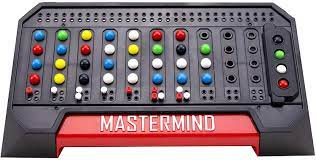
\includegraphics{mm.jpeg}
\end{figure}


\section{Formal Definition}
This game can be formalized as The Mastermind Problem. Given a set of guesses and their corresponding feedback, can we determine what solutions code(s) would produce such behavior? This is effectively a multi-dimensional search problem which has been proven to be NP-Complete\footnote{Stuckman, J., \& Zhang, G. Q. (2005). Mastermind is NP-complete. \textit{arXiv preprint cs/0512049}.}.

\section{Algorithm}
\label{sec:algorithm}
Donald Knuth proposed the "Five-Guess Algorithm\footnote{Knuth, D. E. (1976). The computer as master mind. \textit{Journal of Recreational Mathematics, 9}(1), 1-6.}", which was named as such because it will always determine the correct code using only at most five of the eight allowable guesses. The algorithm works as follows:
\begin{enumerate}[label=\textbf{S.\arabic*}]
	\item Generate all possible codes. Call this $S$, representing the universe of possible codes. Here, $|S| = 6^4 = 1296$.
	\item Create a set of possible solutions $P$. At the start, $P=S$.
	\item Choose an initial guess $g_0$. This can be hard-coded or randomly selected from $P$, as no information about the solution code has been obtained yet.
	\item \label{itm:algo_repeat} Play guess $g_0$ and obtain a response $r$ from the codemaker.
	\item \label{itm:algo_filter} Filter $P$ to remove all codes which could not possibly be the solution based on this response.
		\begin{itemize}
		\item For a code to possibly be the actual solution, its response to $g_0$ must also be exactly $r$.
		\end{itemize}
	\item Select the best next guess $g_1$ from $S$ using a minmax algorithm: minimize the maximum possible number of remaining codes in $P$ after this guess.
		\begin{itemize}
		\item The maximum possible number of remaining codes in $P$ after a guess $g_2$ can be calculated by determining the response of each code in $P$ to $g_2$. The response which appears with the greatest frequency is the worst case (resulting in the largest $P$ after filtering).
		\item In the case of a tie between codes, prefer a code which is still a possible solution, i.e. it is in $P$. As a final tiebreaker, select the numerically lowest code.
		\end{itemize}
	\item Repeat from \autoref{itm:algo_repeat} with guess $g_1$. Repeat until the solution is found ($|P|=1$).
\end{enumerate}

\section{Extension}
It is desirable to increase the computational difficulty of the problem so as to produce more reliable timing results. A program running over a longer amount of time will allow for recorded times to be more robust against random noise. As such, we increase the search space of the algorithm by extending the game to use $c$ colors and $h$ holes (previously, $c=6$ and $h=4$). As such, the universe of codes expands: $|S| = c^h$. For performance analyses in the remainder of this report, $c=10$ and $h=4$ are selected, resulting in $|S| = 10,000$.

\section{Sequential Implementation}
Segments of the sequential implementation are highlighted within this section. For a full code listing, see the Appendix. %TODO: Link
Among other things, the appendix includes code allowing a human codemaker to play against the algorithm. 

\subsection{Datatypes}
\begin{minted}{haskell}
type ResponsePegs = (Int, Int) -- (#black, #white)
\end{minted}
The response providing feedback about a code is presented as a pair consisting of the number of black pegs and number of white pegs in the response.

\begin{minted}{haskell}
type Code = [Int]
\end{minted}
A code is a collection of colored pegs. Each peg is an $Int$ which correponds to a color in set $[1..c]$.

\begin{minted}{haskell}
type Possibility = (Int, Bool, Code) -- (Score, Invalid, Code)
\end{minted}
A $Possibility$ is a candidate for the next guess. The score represents the size of $P$ after this guess in the worst case. The invalid flag tracks whether the code is a possible solution (in $P$) or not. Note that finding the minimum $Possibility$ will perform the next guess selection process including tiebreakers as described in \autoref{sec:algorithm}.

\subsection{Generating a Response}
\begin{minted}{haskell}
guessResult :: Code -> Code -> ResponsePegs
guessResult ans guess = (numBlack, numWhite)
    where numBlack = length $ filter id $ zipWith (==) ans guess
          numWhite = sum (map minCodeCount $ nub guess) - numBlack
          minCodeCount v = min (count v ans) (count v guess)
          count v ls = length $ filter (==v) ls
\end{minted}
The number of black pegs ($numBlack$) can be calculated by looking for pegs in the same position with the same color. For determining the number of white pegs ($numWhite$), each color is iterated over. The minimum number of times that color appears in both codes corresponds to the number of white pegs that color will generate (e.g., three green pegs in the guess and two green pegs in the solution means two white pegs are generated). However, the number of black pegs must be subtracted from this sum (as if a peg is both the right color and in the right position, it will generate a black peg \textit{instead} of a white peg).

\subsection{Scoring a Candidate Guess}
\begin{minted}{haskell}
scoreGuess :: CodeSet -> Code -> Possibility
scoreGuess possible code = (score, valid, code)
    where
        valid = code `elem` possible
        allResponses = map (guessResult code) possible
        score = getMaxCount allResponses
        getMaxCount xs = maximum $ map snd $ getCounts xs
        incCount o [] = [(o, 1)]
        incCount o (x@(v, c) : xs)
            | v == o = (v, c + 1) : xs
            | otherwise = x : incCount o xs
        getCounts xs = foldr incCount [] xs
\end{minted}
TODO: explain

\subsection{Filtering the Possible Set}
\begin{minted}{haskell}
filterCodeSet :: CodeSet -> Code -> ResponsePegs -> CodeSet
filterCodeSet set guess response =
    filter ((response ==) . guessResult guess) set
\end{minted}
TODO: explain

\subsection{Playing the Game}
\begin{minted}{haskell}
playMastermind ::  Code -> Code -> Int -> CodeSet -> CodeSet -> IO Int
playMastermind guess solution k fullSet possibleSet = do
  putStrLn $ "Guessing: " ++ show guess
  let response = guessResult guess solution
  putStrLn $
    "Response: " ++ show (fst response) ++ " black and "
      ++ show (snd response)
      ++ " white"
  let possibleSet' = filterCodeSet possibleSet guess response
  if length possibleSet' == 1
    then do
      putStrLn $ "Solved: " ++ show (head possibleSet')
      return (k + 1)
    else do
      let possibilities = map (scoreGuess possibleSet') fullSet
      let (_, _, nextGuess) = minimum possibilities
      playMastermind nextGuess solution (k + 1) fullSet possibleSet'
\end{minted}
TODO: explain

\subsection{Performance}
TODO: show performance with the two codes
\subsection{Fixing that Bump}
% https://stackoverflow.com/questions/40948153/find-min-elements-index-of-a-large-list-in-haskell
% This will fix it: note that we will have to get timings for all the combinations again after this if it has a substantial effect

\section{Parallelization}
TODO: what we tried for parallelization, results, etc.
\subsection{parMap}
TODO: parMap each code comparison (too many sparks); then parMap each candidate code
TODO: I think we should try to fix the bug or leave it out for the one that ran 8 CPUs but only on one of them. it's also just parMap so don't expect it to be very different.
TODO: table showing numthreads vs. performance, line graph
\subsection{Chunks}
TODO: chunks, table showing numchunks vs. performance, line graph, 2 or 3 screenshots showing load balancing improving as number of chunks increases


\section{Conclusion}
TODO: bar graph showing different methods, discussion of which one was fastest

\section{References}

\section{Appendix: Code}

\end{document}
